\documentclass[conference]{IEEEtran}
\IEEEoverridecommandlockouts
% The preceding line is only needed to identify funding in the first footnote. If that is unneeded, please comment it out.
\usepackage{cite}
\usepackage{amsmath,amssymb,amsfonts}
\usepackage{algorithmic}
\usepackage{graphicx}
\usepackage{textcomp}
\usepackage{xcolor}
\def\BibTeX{{\rm B\kern-.05em{\sc i\kern-.025em b}\kern-.08em
    T\kern-.1667em\lower.7ex\hbox{E}\kern-.125emX}}
\begin{document}

\title{RICE CARMA\\

}

\author{\IEEEauthorblockN{Fredrick Chiu, Tsung-Yu Liu, Varun Santhosh}
\IEEEauthorblockA{\textit{Department of Electrical and Computer Engineering} \\
\textit{Rice University}\\
Houston, Texas, USA \\
fc51@rice.edu, tl152@rice.edu, vs70@rice.edu \\
github: https://github.com/FredRISC/CARMA}
%%\and
}

\maketitle

\begin{abstract}
This report presents the midterm progress of a project aimed at evaluating parametrized Systems-on-Chip (SoCs) integrated with a Vector Processing Unit and a Deep Neural Network (DNN) accelerator within the Chipyard framework. The Chipyard platform provides an open-source, customizable environment for SoC design and analysis, leveraging generators such as Rocket, Saturn, and Gemmini. Our goal is to optimize performance and shared workloads by combining vector processing capabilities with DNN acceleration. We detail the methodology for hardware configuration, simulation, and partial results obtained using cycle-accurate simulators. Preliminary findings demonstrate the feasibility of integrating these components with minimal RTL changes, showcasing promising performance metrics. Future work will focus on refining configurations for optimal power, performance, and area (PPA) trade-offs.
\end{abstract}

\begin{IEEEkeywords}
SoC, RISC-V, RVV, Chisel
\end{IEEEkeywords}

\section{Introduction}
The demand for efficient SoC designs has grown significantly due to the increasing complexity of computational workloads in applications such as machine learning and signal processing. Open source frameworks supporting RISC-V ISA have been emerging for the last 10 years, e.g. Princeton OpenPiton and PULP from ETH Zurich, but Chipyard from UC Berkeley as a Chisel-based generator-based SoC framework takes advantage of the benefits of the Scala programming for enhanced RTL design. This project aims to evaluate parametrized SoCs that integrate a Vector Processing Unit (Saturn) and a DNN accelerator (Gemmini) for enhanced performance within the Chipyard framework. Chipyard is an open-source platform, offering tools for flexible hardware-software co-design. By leveraging its parameterizable features, we aim to create custom configurations that address workload sharing between scalar cores and accelerators while minimizing design invasiveness. 



\section{METHODS}
Everything starts from a generator configuration, where generators are written in Chisel. Generators are also capable of integrating third party Verilog instance IP as shown in fig1. RTL build process focuses on elaboration and transformation of the base generators. FIRRTL - IR enables automated manipulation of the hardware description.

\subsection{Chipyard}


\begin{figure}[htbp]
\centerline{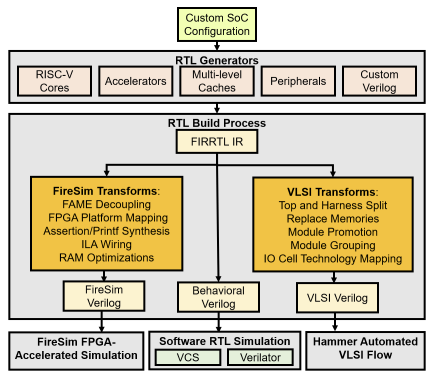
\includegraphics{Chipyard.png}}
\caption{High-level overview of the Chipyard framework [1]}
\label{fig}
\end{figure}

Design Flows: 
RTL Software Simulation, FPGA-Accelerated Emulation, FPGA Prototyping, VLSI Fabrication

Both FPGA-accelerated and conventional software simulations can be used to confirm and validate the design. The design can then be passed via portable VLSI design routines to produce GDSII data that is suitable for tapeout for a variety of target technologies. Additionally, Chipyard offers a system for managing workloads that creates software workloads for design exercises.
\\\\
Hardware Configuration:
\begin{itemize}
    \item Chipyard framework: Used to configure hardware components such as Rocket Core (5-stage pipelined scalar core), Saturn (vector processing unit), and Gemmini (DNN accelerator).
\end{itemize}
\begin{itemize}
    \item Parameterization: Adjusted hardware parameters like systolic array dimensions, vector register file size, and memory hierarchy settings to explore different configurations.
\end{itemize}
Simulation Tools:
\begin{itemize}
    \item Cycle-Accurate Simulators: Verilator and FireSim were employed to simulate hardware performance under real workloads.
\end{itemize}
\begin{itemize}
    \item Functional Simulators: Spike was used for quick validation of configurations.
\end{itemize}
Software Stack:
\begin{itemize}
    \item Integrated RISC-V binaries for baremetal testing and Linux-based applications. Custom testbenches were developed to evaluate specific features like vector instruction scheduling in Saturn and matrix multiplication in Gemmini.
\end{itemize}

RTL generator
\subsubsection{Rocket Chip}
Rocket is a 5-stage in-order scalar core generator. Rocket Chip includes many parts of the SoC besides the Rocket core itself. The fig.2 shows a dual-core Rocket system. Rocket core is grouped with a page-table walker, L1 instruction cache, and L1 data cache into a RocketTile. For MMIO peripherals, the SystemBus connects to the ControlBus and PeripheryBus. The ControlBus attaches standard peripherals like the BootROM, the Platform-Level Interrupt Controller (PLIC), the core-local interrupts (CLINT), and the Debug Unit.
\begin{figure}[htbp]
\centerline{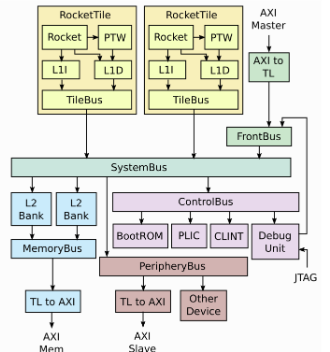
\includegraphics[width=0.3\textwidth]{Rocket chip.png}}
\caption{Block diagram of Rocket chip generator [1]}
\label{fig}
\end{figure}

\subsubsection{Saturn}
Saturn acts as a “vector engine” that executes RISC-V vector instructions alongside a host scalar core[3]. It targets deployment in DSP-like and specialized cores rather than high-end servers, emphasizing configurability 
and compliance with the full RVV standard. It’s a Vector Unit which support RVV ( RISC-V Vector Extension)[3].
\begin{figure}[htbp]
\centerline{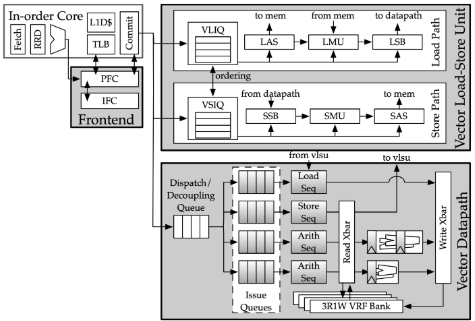
\includegraphics[width=0.4\textwidth]{Saturn.png}}
\caption{Overview of Saturn's Microarchitecture [3]}
\label{fig}
\end{figure}

\subsubsection{Gemmini}
Gemmini is a customizable full stack DNN accelerator generator that enable system level design and evaluation. Most DNN accelerators don't provide integration with host CPUs and shared resources, and hence system level evaluation. It provides customizable hardware template, multi-layered software stack for programmers and system level integration.

\begin{figure}[htbp]
\centerline{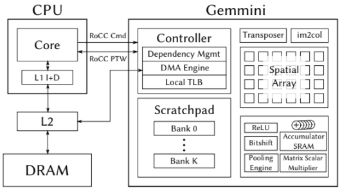
\includegraphics{Gemmini.png}}
\caption{Gemmini hardware architecture template [3]}
\label{fig}
\end{figure}


\section{Discussion}
Here are some potential or temporary challenges and our alternative solutions:\\
\begin{itemize}
    \item Licensing is a serious issue now, e.g. AWS cloud computing platform for FireSim. If this does not work, we will try to use verilator instead.  We will also try to simplify our testbench to make verilator's life easier. 
    \item Saturn is newly released in late 2024 and it is not in the stable branch of the Chipyard github, so whether or not it is compatible with the other generators is a question. In this case, we will instead put more emphasis on analyzing the parametrized Saturn as well as parameterized Gemmini, and reach out to the Berkeley's team for help. 
    \item Evaluations of Performance, Power, and Area (PPA) might not be possible without implementation (e.g. p\&r), and this will require us to go through Hammer VLSI flow in the Chipyard, which is not of our semester goals. In this case, we will try to use the SoC counter or FireSim simulation counter as mentioned in the midterm presentation, to profile the hardware performance of overall SoC or specific components.
\end{itemize}


\begin{thebibliography}{00}

\bibitem{b1} Amid, Alon and Biancolin, David and Gonzalez et al., Chipyard: Integrated Design, Simulation, and Implementation Framework for Custom SoCs, UC Berkeley.

\bibitem{b2} Genc, Hasan, et al. "Gemmini: Enabling systematic deep-learning architecture evaluation via full-stack integration." 2021 58th ACM/IEEE Design Automation Conference (DAC). IEEE, 2021.

\bibitem{b3} Jerry Zhao et al., The Saturn Microarchitecture Manual, UC Berkeley.
\end{thebibliography}
\vspace{12pt}


\section{Ackowledgement}
We acknowledge the support provided by UC Berkeley’s Chipyard development team for their open-source resources and documentation. We also thank Rice University and particularly Professor Ray Simar for their contributions and mentorship to this project.

\end{document}
